%-----------------------------------------------------------------
%	HURRICANE TRACKS DATA
%	!TEX root = ./../main.tex
%-----------------------------------------------------------------
\subsection{Hurricane tracks data sets}\label{sec:hurdat}

\subsubsection{Description of the database}\label{ssec:hurdat-intro}
Although \citeauthor{Corral2010} analyse several ocean basins, we will focus only on the North Atlantic (N.~Atl.) and the Northeast Pacific (E.~Pac.) Oceans. The reason to do this is the abundance of research on these two basins and the precision of the database provided by the National Hurricane Center (NHC)~\cite{o:NHC}: the HURDAT~\cite{o:hurdat2}.

Since both basins directly concern USA territories (especially the N.~Atl.), the government's efforts on improving the tracking and prediction technologies, routine satellite imagery has been used since as early as the late 1960s.

A major change between our data sets and the ones used in \cite{Corral2010} is that the second-generation hurricane database (HURDAT2), has been developed this decade~\cite{Landsea2013}. The improvements of the revised version are mainly:
\begin{enumerate}[(i)]
	\item Inclusion of non-developing tropical depressions.
	\item Inclusion of systems that were added to the database after the end of each season.
\end{enumerate}
Also, the ongoing post-storm analysis reviews of the tropical-cyclones have revised several storms~\cite{o:hurdat-comparison}, particularly important in the 1851--1960 era.

%-----------------------------------------------------------------
\subsubsection{Tropical-cyclones classification}\label{ssec:hurr-class}
Tropical cyclones are classified into three main groups, based on wind intensity: tropical depressions, tropical storms, and a third group of more intense storms, whose name depends on the region. In particular, in the Northeast Pacific or in the North Atlantic, it is called a hurricane. In table~\ref{tab:hurr-class} we can see a detailed classification of the tropical-cyclones studied in this text.
\begin{table}[H]
	\centering
	\begin{tabular}{l c c}
		\toprule
		\toprule
		\multicolumn{1}{c}{Category} & \multicolumn{2}{c}{1--minute sustained winds} \\
		\midrule
		Tropical depression  & $\le \SI{33}{\knot}$      & ($\le \SI{61}{\km/\hour}$) \\
		Tropical storm       & $\SIrange{34}{63}{\knot}$ & ($\SIrange{63}{118}{\km/\hour}$) \\
		Category 1 hurricane & $\SIrange{64}{82}{\knot}$ & ($\SIrange{119}{153}{\km/\hour}$) \\
		Category 2 hurricane & $\SIrange{83}{95}{\knot}$ & ($\SIrange{154}{177}{\km/\hour}$) \\
		Category 3 major hurricane & $\SIrange{96}{112}{\knot}$  & ($\SIrange{178}{208}{\km/\hour}$) \\
		Category 4 major hurricane & $\SIrange{113}{136}{\knot}$ & ($\SIrange{209}{253}{\km/\hour}$) \\
		Category 5 major hurricane & $\ge \SI{137}{\knot}$       & ($\ge \SI{254}{\km/\hour}$) \\
		\bottomrule
	\end{tabular}
	\caption{Tropical-cyclone classification used by the NHC}
	\label{tab:hurr-class}
\end{table}

%-----------------------------------------------------------------
\subsubsection{Importing raw data}\label{ssec:hurdat-import}
The format of the HURDAT2 data sets is documented at~\cite{Landsea2014,Landsea2016}. A record of data is recorded once every 6 hours for each storm (although there are additional records for certain storms). The record is comprised of the date and time, storm identifier, system status (cf. tropical-cyclone category), latitude and longitude of the centre of the storm, the sustained surface wind speed (in knots) observed in the storm, and several other properties we are not interested in.

The data sets used can be downloaded from \url{http://www.aoml.noaa.gov/hrd/hurdat/hurdat2-1851-2016-apr2017.txt} (N.~Atl.) and \url{http://www.aoml.noaa.gov/hrd/hurdat/hurdat2-nepac-1949-2016-apr2017.txt} (E.~Pac.).

\sk
Given the systematic format used by the NHC, it's fairly easy to read the raw data using R (a programming language for statistical computing). First of all, we need to split the data into two lists: (i) metadata (\inline{hurr.meta}) containing the values for the storm ID, name, and number of observations for the storm, and (ii) observations (\inline{hurr.obs}) for each storm record:
\begin{lstlisting}[caption=Read and clean raw data, label=snp:hurdat-read]
# Read and split raw data ----------------------------------
tracks.file <- paste0("data/", filename)
hurr.tracks <- readLines(tracks.file)
hurr.tracks <- lapply(hurr.tracks, str_split, pattern = ",", simplify = TRUE)

# Clean the raw data ---------------------------------------
# Split the hurr.tracks into meta and observation lists
hurr.lengths <- sapply(hurr.tracks, length)
hurr.meta <- hurr.tracks[hurr.lengths == 4]
hurr.obs <- hurr.tracks[hurr.lengths == 21]
\end{lstlisting}

Then we can convert the data into data frames\footnote{The concept of a data frame comes from the world of statistical software used in empirical research; it generally refers to “tabular” data: a data structure representing cases (rows), each of which consists of a number of observations or measurements (columns).} and select only the observations we are interested in, and rename the columns to easily manipulate the data later:
\begin{lstlisting}[caption=Create data frames and select observations, label=snp:hurdat-clean]
# Create and clean meta data frame
hurr.meta <- lapply(hurr.meta, tibble::as_tibble)
hurr.meta <- bind_rows(hurr.meta)

hurr.meta <- hurr.meta %>%
	dplyr::select(-V4) %>%
	rename(storm.id = V1, storm.name = V2, n.obs = V3) %>%
	mutate(storm.name = str_trim(storm.name),
				 n.obs = as.numeric(n.obs))

storm.id <- rep(hurr.meta$storm.id, times = hurr.meta$n.obs)

# Create and clean obs data frame
hurr.obs <- lapply(hurr.obs, tibble::as_tibble)
hurr.obs <- bind_rows(hurr.obs) %>%
	mutate(storm.id = storm.id) %>%
	dplyr::select(storm.id, V1, V2, V4:V7) %>%
	rename(date = V1, time = V2, status = V4, lat = V5, long = V6, wind = V7)
\end{lstlisting}

It is incredibly useful to unite the raw date and time values and convert them into a date-time objects to ease manipulation and calculations. We will also change \texttt{status} to give the levels meaningful names that can be easily understood without consulting the documentation:
\begin{lstlisting}[caption=Change date-time and use meaningful status names, label=snp:hurdat-clean2]
# Change date and time & unite them
hurr.obs <- hurr.obs %>%
	unite(date.time, date, time) %>%
	mutate(date.time = ymd_hm(date.time))

# Meaningful status names
storm.levels <- c("TD", "TS", "HU", "EX", "SD", "SS", "LO", "WV", "DB")
storm.labels <- c("Tropical depression", "Tropical storm", "Hurricane", "Extratropical cyclone", "Subtropical depression", "Subtropical storm", "Other low", "Tropical wave", "Disturbance")
hurr.obs <- hurr.obs %>%
	mutate(status = factor(str_trim(status),
												 levels = storm.levels,
												 labels = storm.labels))
\end{lstlisting}

Ultimately, we want numeric values for the latitude and longitude so that we can use them for mapping and for the SST analysis (\cref{sec:pdi-vs-sst}). Using regular expressions to separate the numeric and non-numeric parts of these columns, it's easy to do this (we won't enter into details; this can be found in the script~\ref{scr:hurdat2_base}, in~\cref{app:code}).

As commented above, there are additional records for certain storms (mainly from aircraft reconnaissance data), but to replicate the methodology used in \cite{Corral2010}, we will just ignore them. We also found that a couple of storms had a middle missing value (\inline{NA} in R, meaning \emph{not available}), so assuming the continuous behaviour of a tropical-cyclone, using Bolzano's Theorem we manually changed them to the corresponding intermediate value:
\begin{lstlisting}[caption=Clean non-standard data and odd middle values for certain storms, label=snp:hurdat-clean3]
# Clean non-standard data ----------------------------------
# Ignore data outside the delta.t = 6 hours
hurr.obs <- hurr.obs %>%
	filter(hour(date.time) == 00 |
					hour(date.time) == 06 |
					hour(date.time) == 12 |
					hour(date.time) == 18) %>%
	filter(minute(date.time) == 00)

# Clean up wind column -------------------------------------
# Manually change odd middle values for AL191976 & AL111973
hurr.obs <- hurr.obs %>%
	mutate(wind = ifelse(storm.id == "AL191976" & wind == " -99", 20, wind),
				 wind = ifelse(storm.id == "AL111973" & wind == " -99", 30, wind),
				 wind = ifelse(storm.id == "AL111973" & month(date.time) == 9 & day(date.time) == 12 & hour(date.time) == 12, NA, wind)) %>%
	filter(is.na(wind) != TRUE)
\end{lstlisting}

One thing to take into consideration is that, even though the use of new technologies improve the best tracks, the uncertainties of the observations are non-trivial. Using aircraft and satellite monitoring data the relative uncertainty of wind speeds falls around $\SI{15}{\percent}$ for tropical storms, $\sim\SI{10}{\percent}$ for category 1 and 2 hurricanes, and $\sim\SI{8}{\percent}$ for major hurricanes~\cite{Landsea2013}.

The inability to work with observational error data does not mean, however, that we won't be able to assign an error to our results. In~\cref{ssec:dpdi} we derive the statistical error of the $PDI$ probability density, whilst for the SST analysis in~\cref{sec:pdi-vs-sst} we will use the standard error of the mean.

%-----------------------------------------------------------------
\subsubsection{Resulting data structure}
In table~\ref{hd:hurdat-head} we show the structure of the \inline{hurr.natl.obs} data frame to illustrate the variables we use in the study (by all means, \inline{hurr.epac.obs} shares the same structure), as well as the format (data type\footnote{In computer science and computer programming, a data type or simply type is a classification of data which tells the compiler or interpreter how the programmer intends to use the data. }) of the observational record data.
\begin{table}[H]
	\centering
	\ttfamily
	\resizebox{\textwidth}{!}{%
	\begin{tabular}{r r r r  r r r r r}
		\toprule
		\toprule
		storm.id & storm.name & n.obs &           date.time &         status &   lat &  long &  wind & storm.year \\
		   <chr> &      <chr> & <int> &              <dttm> &         <fctr> & <dbl> & <dbl> & <dbl> &      <dbl> \\
		\midrule
		AL011851 &    UNNAMED &    13 & 1851-06-25 00:00:00 &      Hurricane &  28.0 & -94.8 &    80 &       1851 \\
		AL011851 &    UNNAMED &    13 & 1851-06-25 06:00:00 &      Hurricane &  28.0 & -95.4 &    80 &       1851 \\
		AL011851 &    UNNAMED &    13 & 1851-06-25 12:00:00 &      Hurricane &  28.0 & -96.0 &    80 &       1851 \\
		AL011851 &    UNNAMED &    13 & 1851-06-25 18:00:00 &      Hurricane &  28.1 & -96.5 &    80 &       1851 \\
		AL011851 &    UNNAMED &    13 & 1851-06-26 00:00:00 &      Hurricane &  28.2 & -97.0 &    70 &       1851 \\
		AL011851 &    UNNAMED &    13 & 1851-06-26 06:00:00 & Tropical storm &  28.3 & -97.6 &    60 &       1851 \\
		\bottomrule
	\end{tabular}}
	\caption{Excerpt of the \inline{hurr.natl.obs} data frame}
	\label{hd:hurdat-head}
\end{table}

%-----------------------------------------------------------------
\subsubsection{Activity windows}\label{ssec:act-windows}
Even though recent improvements have been made to the HURDAT2 database, \cite{o:hurdat-comparison,Landsea2014,Landsea2016}, following the methodology of \citeauthor{Corral2010}, we will intentionally limit this study to the satellite era.

In \cite{Webster2005}, \citeauthor{Webster2005} go into more details about the activity windows for the hurricane tracks data as well as the sea surface temperature used by researchers in the past. In table~\ref{tab:act-windows} we can see a summary of the spatial and temporal activity windows we will use for each basin based on the information available in the previously mentioned papers; we also include the amount tropical-cyclones analysed in the text, $N$, as well as the size of the entire data set, $N_{tot}$.
\begin{table}[H]
	\centering
	\begin{tabular}{l c c c c c c}
		\toprule
		\toprule
		Basin & Years & Season & Longitude & Latitude & $N$ & $N_{tot}$ \\
		\midrule
		N.~Atl. & 1966--2016 & June--October & \ang{90}W--\ang{20}E  & \ang{5}N--\ang{25}N & \num{771} & \num{1756}  \\
		E.~Pac. & 1966--2016 & June--October & \ang{120}W--\ang{90}W & \ang{5}N--\ang{20}N & \num{920} & \num{1071}  \\
		\bottomrule
	\end{tabular}
	\caption{Spatial and temporal activity windows for each basin}
	\label{tab:act-windows}
\end{table}

Below we can see a map for each basin (figures~\ref{fig:map-natl} and~\ref{fig:map-epac}) showing all the storms analysed in the text in red lines, and the spatial window highlighted in green. These maps have been generated by using the function \inline{map_region_hurrs()} defined in the script~\ref{scr:hurdat2_base} in~\cref{app:code}.
\begin{figure}[H]
	\centering
	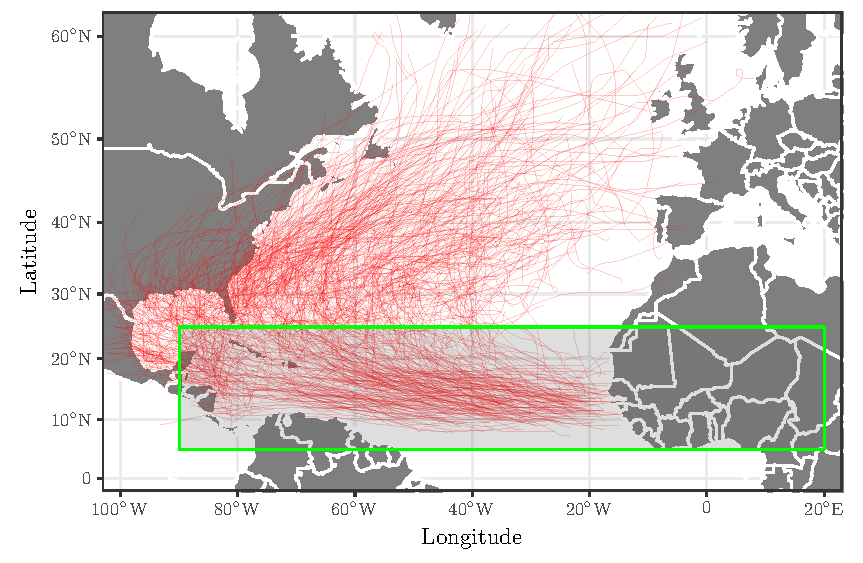
\includegraphics[width=\textwidth]{images/map-natl}
	\caption{Tropical-cyclones best tracks for the North Atlantic Ocean}
	\label{fig:map-natl}
\end{figure}

\begin{figure}[H]
	\centering
	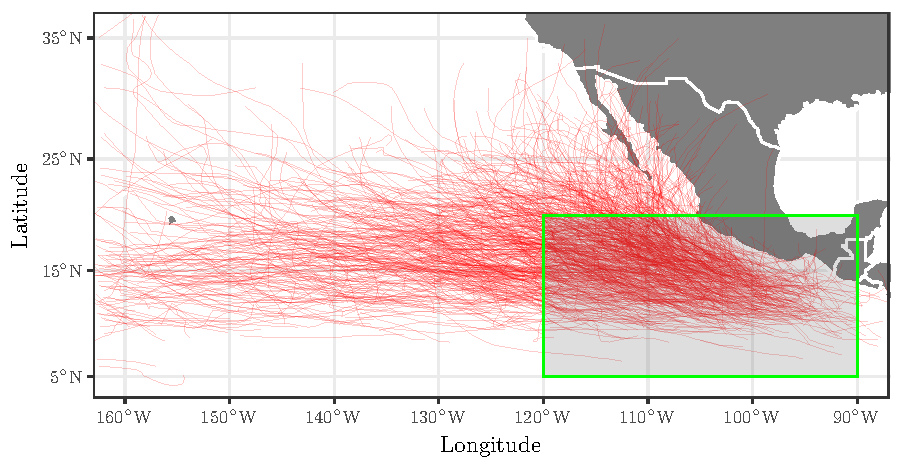
\includegraphics[width=\textwidth]{images/map-epac}
	\caption{Tropical-cyclones best tracks for the Northeast Pacific Ocean}
	\label{fig:map-epac}
\end{figure}
